%\documentclass[CJK]{beamer}
\documentclass{beamer}

\usepackage{amssymb}

\usepackage{latexsym,amssymb,amsmath,amsbsy,amsopn,amstext,color,multicol}
\usepackage{graphicx,wrapfig,fancybox,watermark,picins}
\usepackage{pgf,pgfarrows,pgfnodes,pgfautomata,pgfheaps,pgfshade}
\usepackage{graphics}
\usepackage{movie15}
\usepackage{hyperref}

%\usepackage{CJK}
\usepackage[red,numbers]{beamerthemeHongKong}



\begin{document}
%\begin{CJK*}{GBK}{kai}

\title[Short Title]{Full Title}
\author[Short Author]{Full Author}
\institute[institute]{institute full name}
\date{\today}
\frame{\titlepage}


\section*{Table of Contents}
\frame {
  \frametitle{\secname}
  \tableofcontents
}

\AtBeginSubsection[] {
  \frame<handout:0> {
    \frametitle{Outline}
    \tableofcontents[current,currentsubsection]
  }
}

\section{Section A}

\subsection{Subsection A-A}

\begin{frame}
\frametitle{\subsecname}
  \begin{columns}
  \column{0.5\textwidth}
    \begin{overprint}
    \onslide<1>
      \begin{figure}
      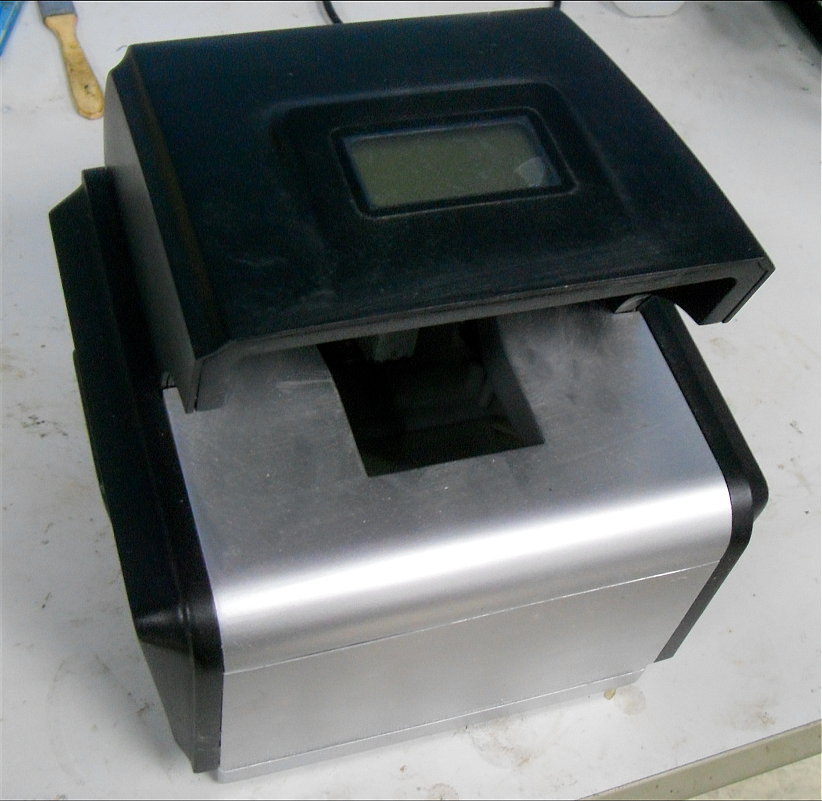
\includegraphics[width=\textwidth]{image/test-image1}
      \caption{figure A}
      \end{figure}
    \onslide<2>
      \begin{figure}
      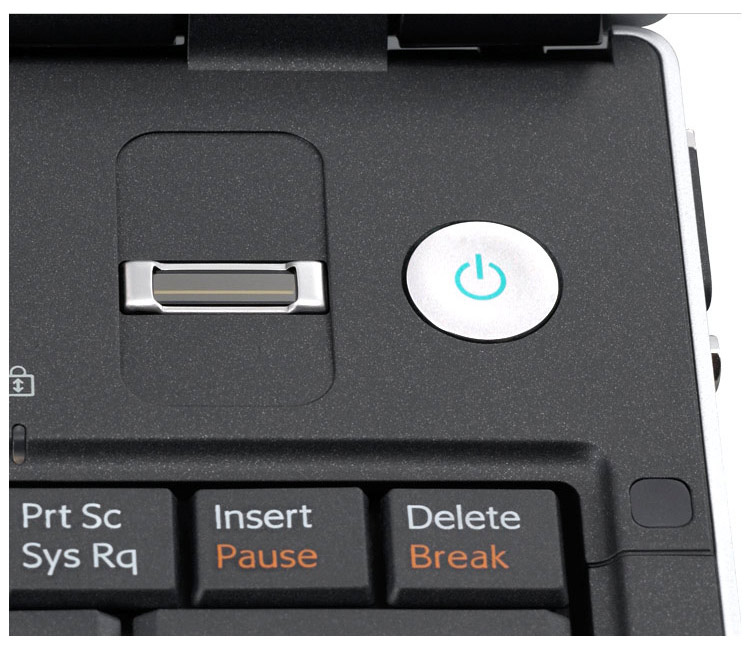
\includegraphics[width=\textwidth]{image/test-image2}
      \caption{figure B}
      \end{figure}
    \end{overprint}
  \column{0.5\textwidth}
    \begin{block}{example}<1->
      \begin{enumerate}
        \item<1-|alert@1>
        text about figure A
        \item<2-|alert@2>
        text about figure B
      \end{enumerate}
    \end{block}
  \end{columns}
\end{frame}

\subsection{Subsection A-B}

\begin{frame}
\frametitle{\subsecname}
    \begin{itemize}[<+- | alert@+>]
      \item
      item A
      \item
      Item B
      \item
      Item C
    \end{itemize}
\end{frame}

\section{Section B}

\subsection{Subsection B-A}

\begin{frame}
\frametitle{\subsecname}
    \begin{enumerate}
      \item
      item A
      \item
      Item B
      \item
      Item C
    \end{enumerate}
\end{frame}

\subsection{Subsection B-B}

\begin{frame}
\frametitle{\subsecname}
    \begin{itemize}
      \item
      item A
      \item
      Item B
      \item
      Item C
    \end{itemize}
\end{frame}

\subsection*{Thanks}

\begin{frame}
\frametitle{\subsecname}
  \begin{columns}
  \column{2.5cm}
  \column{5cm}
    \Huge{Thank you!}
  \column{2.5cm}
  \end{columns}
\end{frame}

%\end{CJK*}
\end{document}
